% Chapter 5 implementation

\chapter{Implementation} % Main chapter title

\label{Implementation} % For referencing the chapter elsewhere, use \ref{Chapter1} 

\section{Architecture}
\begin{figure}
\centering
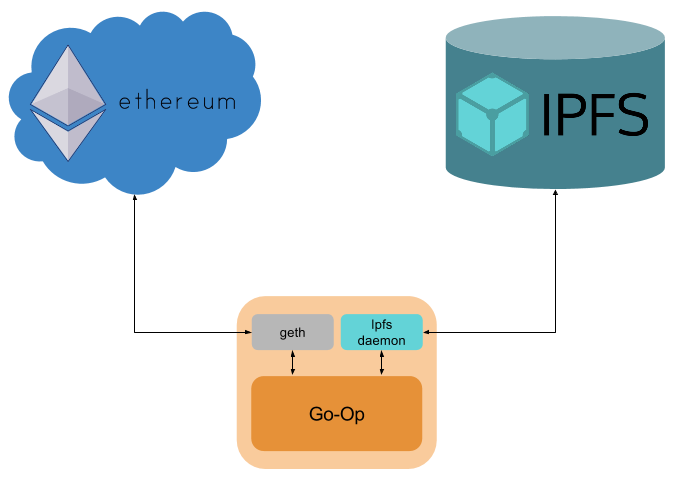
\includegraphics[width=\textwidth]{Figures/GoopArch}
\decoRule
\caption[]{}
\label{fig:GoopArch}
\end{figure}

Figure \ref{fig:GoopArch} is a high level illustration of the Go-Op application architecture. It is a simple distributed architecture and notable for the lack of any client server asymmetry. The Ethereum cloud represents the Ethereum peer to peer network and the large IPFS database represent the IPFS network similarly. The 'host machine' must run both an Ethereum and IPFS client in order to participate in the respective networks. The Go-op application is a typical javascript/HTML/CSS web application and can therefore be run in a normal Internet browser. \\

Go-op is very much a proof of concept application and currently requires the manual installation of both an Ethereum and IPFS client. Users are not generally expected to engage in such low level technical processes but it is practical limitation for the time being. The idealised Web3 architecture (discussed in section \ref{sec:web3Arch}) outlines a better vision for user interaction with new tools such as the Mist browser which is planned to be released later this year. In figure \ref{fig:GoopArch} Mist would be represented by the light orange box surrounding the host processes. The Mist browser will internally manage the Web3 clients to hide unnecessary complexity from the application users. \\

The Go-op 'front end' code interacts with the local Ethereum node through the web3.js library\cite{Web3JS}. The web3.js library implements the Web3 Javascript API\cite{JavascriptAPI} which is well documented online (see ref). Under the hood, the web.js library communicates with the local Ethereum instance via RPC (remote procedure calls). Communication between Go-op and the IPFS client is achieved through the ipfs-js\cite{ipfs-js} library, developed by ConsenSys (a leading blockchain technology company developing on Ethereum). The ipfs-js library is a simple wrapper around official ipfs client javascript library but adds some nice Ethereum specific utilities such as conversions between hex (format for Ethereum storage) and base58 format of Ipfs addresses. \\

One important note is that user accounts are not managed through the web3 library and must be added / removed etc through the Ethereum client command line interface. User accounts need to be unlocked before they can be used by the Go-op application to sign transactions. Again, the development of new user friendly interfaces will soon make it possible to avoid such pains. \\

For more information about installing and running Ethereum and IPFS clients consult Appendix A. \\

A possible alternative to running Web3 clients locally is to run them as web services (this is the kind of approach offered by Block apps\cite{BlockApps} for example). Whilst this has the potential to simplify the problem in the short term, it generally works against the objectives of decentralisation. The process introduces the web service as a 'trusted' intermediary. It is counter intuitive to add points of trust into the process of executing Ethereum contracts as the whole point is to eliminate 'centralised trust' in the first place. \\

Lower level architecture explanations for the Go-op application and smart contract system are provided in the following sections. \\

\section{Go-op Smart Contract System}
The smart contract system for Go-op (Figure \ref{fig:SCArch}) is relatively small. It is composed of five static contract accounts (CMC, UserController, UserRegistry, CoopRegistry and MembershipRegistry) and a dynamic number of user and CoopContract accounts. The architecture of the contracts roughly follows the Five Types design pattern discussed in section \ref{sec:scDesign}.\\ 

The principal entities in the system are users and 'coops' which are stored in the UserRegistry contract and CoopRegistry contract respectively. The many to many 'membership' relation between users and coops is stored by the MembershipRegistry contract. The next few subsections explain the role of each system component in detail.\\

\begin{figure}
\centering
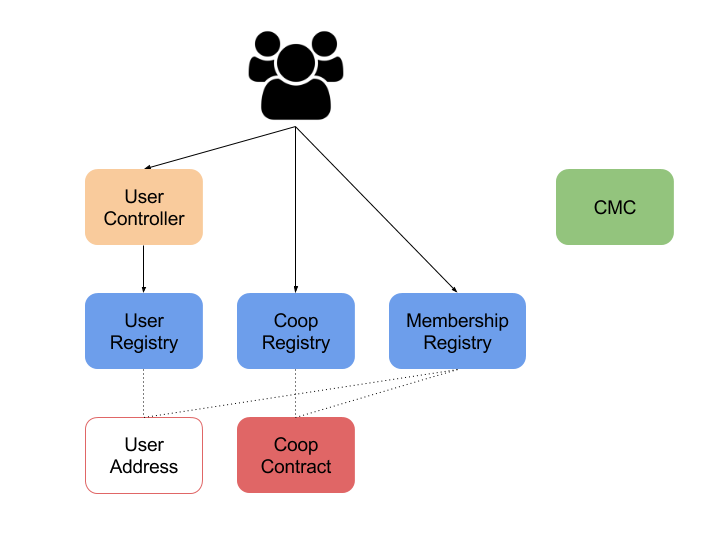
\includegraphics[width=\textwidth]{Figures/SCArch}
\decoRule
\caption[]{}
\label{fig:SCArch}
\end{figure}

\subsection{CMC}
Although it was not possible to fully realise the Five Type design pattern due to practical limitations (discussed shortly), Go-op still makes use of a CMC (contract management contract) to help manage modularity and permissions. Essentially, the CMC holds a mapping of component names to contract addresses. Only the owner of the CMC, that is the account that created it, is able to add, remove and 'dissolve' contracts. The CMC contract is a standard component of the Five Types pattern. For a code listing and detailed explanation see the Eris Industries tutorial \cite{FiveTypes}.

\subsection{CMCEnabled}
CMCEnabled is an 'abstract' contract that is inherited by all non CMC contracts. It defines a minimal interface required by the CMC to interact with non CMC contracts. A ContractProvider contract is used to define the minimal interface required in the opposite direction. Again, these are also standard contracts of the Five Types pattern. A code listing and detailed explanation be found here\cite{FiveTypes}.\\

\subsection{UserRegistry \& UserController}
The UserRegistry contract (Figure \ref{fig:UserRegistry}) is very simple. It stores a mapping of user account addresses to IPFS addresses and has two functions, setUserData and getUserData (not shown in figure), for reading and writing to this mapping. The UserRegistry uses the CMC contract to restrict both read and write permission to only the UserController contract. \\

\begin{figure}
\centering
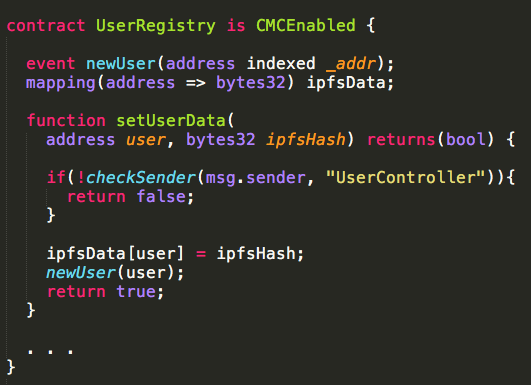
\includegraphics[width=\textwidth]{Figures/UserReg2}
\decoRule
\caption[]{Snippet of the UserRegistry contract}
\label{fig:UserRegistry}
\end{figure}

The UserController is, for now, simply a wrapper for the UserRegistry contract. It does not provide any additional logic and was included in an attempt to follow the Five Types pattern (section \ref{sec:scDesign}). Although it is a redundant component, the process of adding a user controller to the system revealed some practical limitations to composing smart contract systems. Critically, the possible return types between contracts executing in the EVM are different to the returnable types for external calls. To be specific, variable length arrays, which includes strings and byte arrays, are not possible return types between contracts executing within the EVM but are permitted return types for direct calls from externally owned accounts. \\

Because IPFS addresses are 34 bytes long and the largest fixed size byte array in Solidity is 32 bytes, it is not possible to pass a whole IPFS address between the UserRegistry and the UserController contracts. This is a big issue for dapps that use IPFS but also want to follow modular design patterns that require contract interaction. \\

There are a few possible 'workarounds' in this case:\\

\begin{enumerate}[label=(\alph*)]
\item Remove the UserController completely and read straight from the registry. From a design perspective this is a somewhat degenerate solution. \\

\item Add logic to the UserController that splits and re-combines the IPFS hash on saving and retrieving from the UserRegistry. This would require the UserRegistry to implement two methods for returning different parts of the IPFS hash e.g \code{first32\allowbreak IPFSbits()}, \code{next2\allowbreak IPFSbits()}. This is not an ideal solution because adding processing to deconstruct and reform byte arrays in the UserController would increase the gas requirements and therefore the costs of the system. \\

\item Only store the last 32 bytes in the blockchain. This is possible because IPFS hashes are 'self-describing' and the first 2 bytes just defines the hash function used. For all current intents and purposes this is always SHA-256. The hex string that represents SHA-256 within IPFS, '0x1220', is simply dropped and re-appended on writing and reading from Ethereum. This is an easy to implement solution and is the workaround currently employed by Go-op for the UserController and UserRegistry. However, it only works in this specific case for IPFS addresses and doesn't solve the dynamic array return type problem in general.\\
\end{enumerate}

There are plans to implement dynamic return types between contracts in a future protocol update so, hopefully, the current workaround is only temporary\cite{ReturnArray}. A big factor for choosing workaround c) is that it will be the easy to revert once the protocol is updated.\\

\subsection{CoopRegistry}
The CoopRegistry is another relatively simple contract. It stores the addresses of all CoopContract contracts in the Go-op system. Unlike the UserRegistry it does not store any additional information about cooperatives, such as an IPFS address, because this is stored by the individual CoopContracts themselves. The CoopRegistry contract exposes two methods: \code{newCoop()} and \code{getCoops()}. \\

\code{getCoops()} returns the state variable array of CoopContract addresses. \\
 \begin{figure}
\centering
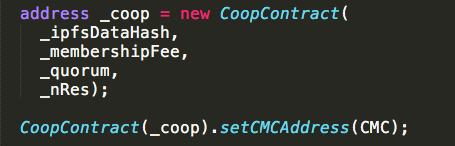
\includegraphics[width=\textwidth]{Figures/CoopRegistry}
\decoRule
\caption[]{Snippet of the CoopContract creation within the CoopRegistry contract (a Solidity definition for CoopContract must be provided in order to compile CoopRegistry) }
\label{fig:CoopRegistry}
\end{figure}

\code{newCoop()} creates a new instance of a CoopContract with the provided parameters (see Figure \ref{fig:CoopRegistry}) and saves the resultant address in the registry array.\\

A cleaner 'separation of concerns' might be achieved here by extracting the complexity of CoopContract creation out of the CoopRegistry into a CoopController. This could help modularity by creating a more rigid API for the CoopRegistry and would abstract the registry contract from the public facing API. However, assuming the avoidance of intensive contract code[Footnote] it is not possible to pass variable length arrays, such as the list of coop addresses, between contracts. This means that at least some part of the public facing API must be exposed by the CoopRegistry directly. At present therefore, a new coop controller contract probably does not simplify the design of the system enough to warrant its introduction. \\

The CoopRegistry does not currently implement a \code{removeCoop()} function. Whilst this may be desirable in future, at present, the precise conditions for removing a coop from the Go-op system are not well understood. \\

\subsection{MembershipRegistry}
The MembershipRegistry contract maintains the many to many 'membership' relationship between users and cooperatives. It is slightly more involved than the other registry contracts as it stores more information, handles more advanced queries and needs to manage payment of membership fees. Figure \ref{fig:MemRegVars} illustrates the state variables of the MembershipRegistry. The relationship is stored in both directions to reduce computation when retrieving membership information. \\

\begin{figure}
\centering
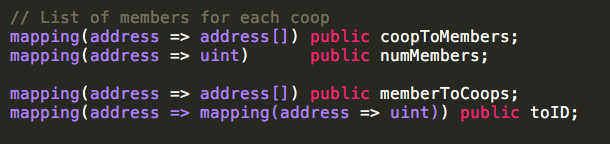
\includegraphics[width=\textwidth]{Figures/MemRegVars}
\decoRule
\caption[]{ }
\label{fig:MemRegVars}
\end{figure}

The MembershipRegistry has five methods \code{register()}, \code{deregister()}, \code{getMembers()}, \code{getCoops()}, \code{idOf()}, \code{totalMembers()} and \code{isMember()}. \\

\code{register()} stores a new relationship between a user and a coop. Registration is successful after a number of checks are completed:
\begin{enumerate}
\item Check with the UserRegistry and CoopRegistry that the calling account is a registered user and that the address of the coop being joined is a CoopContract within the Go-op system.

\item Read the membership fee from the CoopContract of the cooperative being joined. If the value sent with the transaction is not exactly equivalent to the fee then an exception is thrown which causes the inexact fee to be returned to the sender. 

\item Check the member is not joining twice by iterating through all the coops already associated with a member.

\item Forward the membership fee to the CoopContract being joined.

\item Finally, the registry data is updated to reflect the new membership.
\end{enumerate}

The \code{deregister()} method removes the sender as a member of the given coop. In future it is likely that more complex de-registration functionality will be required such as membership termination by group consensus.\\

\code{getMembers()} and \code{getCoops()} are explicit methods for accessing the registry data structs. Again, the need to return variable length arrays removes the practical possibility of a MembershipController contract at this time. \\

The \code{isMember()} method is required by CoopContracts to establish membership during voting.\\

\subsection{CoopContract}
Each cooperative in the Go-op system exists as a unique CoopContract (full listing in section X). The CoopContract is by far the most complex contract because it implements a proposal voting system. The  contract has twelve methods: \code{set\allowbreak CoopData()}, \code{get\allowbreak CoopData()}, \code{get\allowbreak ProposalData()}, \code{get\allowbreak VotesFor()}, \code{getVotes\allowbreak Against()}, \code{has\allowbreak Passed()}, \code{has\allowbreak Failed()}, \code{isA\allowbreak Member()}, \code{getNum\allowbreak Members()}, \code{new\allowbreak Proposal()}, \code{support\allowbreak Proposal()}, \code{close\allowbreak Proposal()}. The majority of these methods are one liners and fairly self explanatory. The most involved functions are \code{new\allowbreak Proposal()}, \code{support\allowbreak Proposal()}, \code{close\allowbreak Proposal()} which will be discussed presently.\\
\begin{figure}
\centering
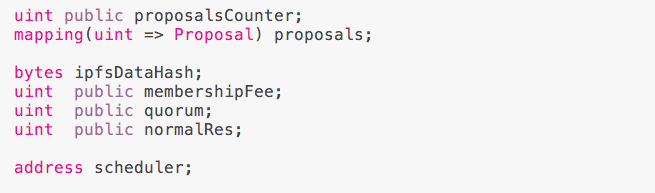
\includegraphics[width=\textwidth]{Figures/CoopState}
\decoRule
\caption[]{ }
\label{fig:CoopState}
\end{figure}

Figure \ref{fig:CoopState} shows the state variables of a CoopContract. The ipfsDataHash holds an IPFS address for non logic-critical information (such as terms and conditions). The membership fee is stored in Wei (a sub denomination of Ether) and the quorum, normal resolution and extraordinary resolution levels are all stored as percentages (integers between 0 and 100). Proposals are stored in the proposals mapping. Figure \ref{fig:ProposalStructs} shows the Proposal and ProposalVotes structs. The textual information for a proposal is also stored in IPFS and it's address is stored in the Proposal struct.\\

\begin{figure}
\centering
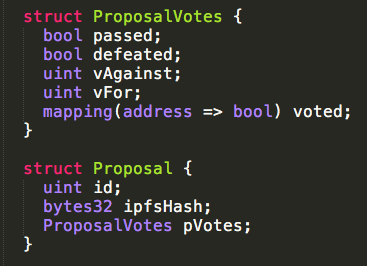
\includegraphics[width=\textwidth]{Figures/ProposalStructs}
\decoRule
\caption[]{ }
\label{fig:ProposalStructs}
\end{figure}

Proposals are created through the \code{newProposal()} method. The process of this method can be broken down into three stages: 
\begin{enumerate}
\item First, it checks the caller is a member of the cooperative via a call to the \code{isMember()} function of the \keyword{MembershipRegistry}. If the caller is not a member then the function call returns immediately. 
\item Secondly, it creates a new Proposal struct from the provided arguments and adds it to the proposals mapping with a new id taken from the proposalsCounter. 
\item Finally, and most interestingly, it schedules a call with the Ethereum alarm clock service to close the proposal at a future block. When the given block number is reached, the Ethereum Alarm Clock service will call the \code{closeProposal()} method on the \keyword{CoopContract}. The Ethereum Alarm Clock service and the challenge of measuring time on a blockchain is discussed at greater depth in section \ref{sec:blocktime}
\end{enumerate}

Votes for proposals are registered with the \code{supportProposal()} function. The behaviour of this function can also be broken down into three stages:
\begin{enumerate}
\item First, it follows the same process as \code{newProposal()} to check the caller is a member of the cooperative.
\item Secondly, it checks if the proposal has not already ended and that the sender has not already voted. If either are true, the function returns.
\item Finally, based on the call parameters, it registers the vote by incrementing either the vFor or vAgainst field of the proposal.\\
\end{enumerate}

The \code{closeProposal()} function is used to close a proposal and determine whether it has passed or been defeated. As described in the description for \code{newProposal()}, this function is triggered by the Ethereum Alarm Clock service. The function proceeds as follows:
\begin{enumerate}
\item The member count is retrieved from the \keyword{MembershipRegistry}. 
\item If the proportion of votes to member count does not surpass the quorum level (see ) then the proposal is closed as defeated. 
\item If quorum is reached and the proportion of 'votes for' to total votes surpasses the normal resolution level (see ) then the proposal is closed as passed, otherwise it is defeated.
\end{enumerate}

In future, the proposal system of the CoopContract could be extended to also allow coops to pass proposals that change the rules of the coop itself (such as the normal resolution level). A new extraordinary resolution level would be required to pass these kinds of special proposals.\\

\section{Client Application}
\subsection{Meteor Framework}
As discussed in 'idealised Web3.0 architecture' (Section \ref{sec:web3Arch}), the 'front end' of an Ethereum dapp is typically built with the same technology stack as that of a traditional web application and therefore is very much compatible with existing browsers. Despite this, a number of popular dapp specific framework choices have emerged from the community (such as Embark\cite{Embark}, Truffle\cite{Truffle} and Meteor\cite{Meteor}) which supposedly offer added usability for Ethereum development (such as integration of test harnesses for Solidity smart contracts). A certain amount of time was necessarily dedicated to the exploration of these frameworks during the initial stages of Go-op development. More information about this investigation can be found in Appendix A.\\

The framework chosen for the development of Go-op was Meteor\cite{Meteor}. Meteor is a 'full stack' javascript application platform that includes a 'key set' of technologies and libraries and a dedicated build tool. The distinguishing feature of the Meteor platform is its emphasis on SPAs (Single Page Applications) and data on the wire, which helps developers easily manage data collections across the client and server. The motivation for using Meteor was based on its popularity within the community (used by established projects including Boardroom see \ref{subsec:boardroom}), the number of supporting libraries and boilerplates and recommendations from Ethereum developers\cite{MeteorRef}.\\

Meteor has recently updated from version 1.2 to 1.3. The update changed the behaviour of the build tool and introduced support for ES2015 modules and npm packages out of the box. Go-op has been developed with Meteor 1.3 in order to future proof as much as possible and embrace the improved compatibility with ECMAScript 6.\\

\subsection{Application Structure}
\begin{figure}
\centering
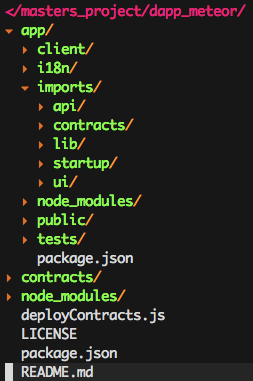
\includegraphics[width=\textwidth]{Figures/AppStructure}
\decoRule
\caption[]{ }
\label{fig:AppStructure}
\end{figure}

Figure \ref{fig:AppStructure} shows the main folders in the Go-op project. This is a typical Meteor 1.3 organisation and should be easily navigable to any developer familiar with the Meteor stack. The role of the various project folders within the app folder are as follows: \\

\begin{itemize}
\item \keyword{client} - name sensitive folder used by the meteor build system.
\item \keyword{I18n} - used by meteor package to enable easy internationalisation of application.
\item \keyword{Imports} - main folder that contains bulk of client side logic. 
\begin{itemize}
\item \keyword{api} - contains database modules and event reactors that form an abstraction layer between the template or view logic and the Ethereum and IPFS interaction code.
\item \keyword{contracts} - This is the destination folder for the compiled 'contract modules' that are generated as part of the deployment script see \ref{subsec:deployScript}.
\item \keyword{lib} - some internal and external library code.
\item \keyword{startup} - common meteor folder. Holds key application files including startup logic and front end routes.
\item \keyword{ui} - contains the template files for the application views.  
\end{itemize}
\item \keyword{contracts} - Contains solidity smart contracts.
\item \keyword{deployContracts.js} - script for compiling, building and deployment of smart contracts see \ref{subsec:deployScript}.
\end{itemize}

Node\_modules, readme and package.json are standard javascript application assets. More information about the Meteor build system and conventions can be found in the guides, tutorials and documentation available at the meteor website.\\

\subsection{API}
This section describes the contents of the api folder which forms a layer between the application view logic and the Web3 'backend'.

\subsubsection{database}
The client side 'database' (as shown in figure X) abstracts complexity away from view logic by orchestrating the retrieval of data from the Web3 'backend' and exposing an easy to use, reactive and 'promisified' interface.\\

\begin{figure}
\centering
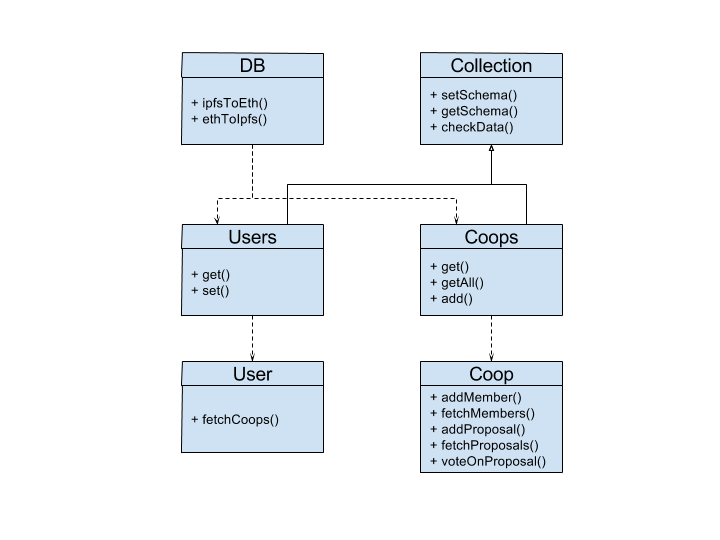
\includegraphics[width=\textwidth]{Figures/dbClassDiagram}
\decoRule
\caption[]{ }
\label{fig:dbClassDiagram}
\end{figure}

Figure \ref{fig:dbClassDiagram} shows the components of the database and the relationship between them. Listing \ref{lst:label} illustrates the API exposed to the view logic. Under the hood, the query first fetches the information for the coop at 'coopAddress' from the smart contract system and then uses it to consruct an in memory \code{Coop} object which it returns. \code{fetchMembers()} triggers another call to the smart contract backend to fill in all the information for a cooperatives members. The \code{Coop} object saves this information internally and then returns a reference to itself. \\

\begin{lstlisting}[caption={Example query to the front end database api}, label={lst:label}]
db.coops.get(coopAddress).then(function(coop) {
	return coop.fetchMembers();
}).then(function(coop) {
	// do something.
});
\end{lstlisting}

The \code{db} class is the entry point of the API. It creates an IPFS connection which it uses to construct the two database collections: \code{Users} and \code{Coops}. The \code{db} class constructs each of the Ethereum 'reactor classes' (discussed in the next section) which are also injected into the two collections. The \code{db} class has two helper functions for converting IPFS addresses between IPFS and Ethereum compatible formats.\\

\code{Collection} is an 'abstract' class that defines some common functionality for a collection, such as setting and checking schemas. Although there is no relational database per se, Go-op still uses schemas to avoid storing malformed data in the Web3 backend. Using schemas to validate on write avoids the need for excessive guard code upon reading, which is typically a more frequent operation.  Go-op uses the js-schema\cite{jsSchema} library for this purpose.\\

The design of the database api is partly inspired by Martin Fowler's Active Record pattern\cite{ActiveRecord} whereby tables and records from a relational database are reflected by in memory objects. The \code{Coops} and \code{Users} collections both implement a \code{get()} method which gathers the information from Ethereum and IPFS and then uses it to construct and return either a \code{Coop} or \code{User} object. \code{Coop} and \code{User} objects have an address field and correspond to real Ethereum accounts. They also have methods such as \code{fetchMembers()} or \code{fetchCoops()} which retrieve additional information from the 'backend' to 'fill in' the objects further.\\

Currently, the \code{Coops} and \code{Users} collections don't implement any level of caching. This means that every time the \code{get()} function is called the data is re-fetched from the Web3 backend. Caching database collections would improve the performance and user experience of Go-op but introduces additional challenges surrounding data consistency and cache invalidation.\\

Figure X illustrates the basic process of collecting data from Ethereum and IPFS. IPFS addresses are retrieved from Ethereum using the web3.js library and the compiled contract modules created by the deployContracts script (see section \ref{subsec:deployScript}). The IPFS address is then converted back into an IPFS friendly format and finally, the data is retrieved from IPFS (via the ipfs-js library) and used to construct in memory objects.\\

\subsubsection{Ethereum Reactors}
In order to explain the role of the \code{EthereumReactor} classes it is necessary to go into a brief aside about reactivity in Meteor. In this context, reactivity describes the ability of the application UI to automatically react or respond to changes in the underlying application data.\\

The native Meteor system follows a transparent reactive programming pattern. The reactive programming pattern can be understood as the interplay between reactive data sources, such as database queries, and reactive data consumers or reactive computation contexts. Reactive data sources record the computation context they are being accessed within. When the value of a reactive data source changes, such as the result of a database query, it triggers all its dependencies which causes all the computation contexts that access the reactive data source to re-run. For a more detailed explanation of transparent reactive programming in Meteor see \cite{Tracker}.\\

To help build reactive user interfaces in Go-op, the database is implemented as a reactive data source. This means that database queries in view templates (listing \ref{lst:label} for example) get re-run whenever the result of the query changes. The result of a query changes whenever data in the backend Ethereum contracts change. The role of the 'reactor classes' is to store dependencies created by database queries and trigger them when changes in Go-op smart contracts are detected. Changes to smart contracts are detected following the event pattern described in section \ref{subsec:events}. \\

\begin{figure}
\centering
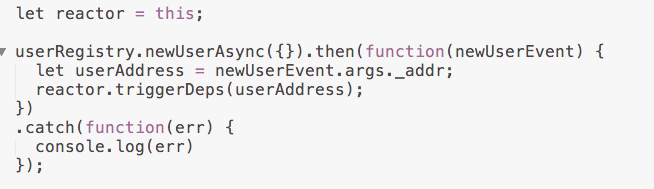
\includegraphics[width=\textwidth]{Figures/UserRegistryReactor}
\decoRule
\caption[]{Critical section of UserRegistryReactor}
\label{fig:UserRegistryReactor}
\end{figure}

When a new user is added to a the \code{UserRegistry} the \code{newUser} event is fired (see Figure \ref{fig:UserRegistry}). Figure \ref{fig:UserRegistryReactor} shows the critical logic in the \code{User\allowbreak Registry\allowbreak Reactor} that listens for this event. When it fires, the \code{UserReactor} triggers all the reactivity dependencies that have been registered to it. \\

\begin{figure}
\centering
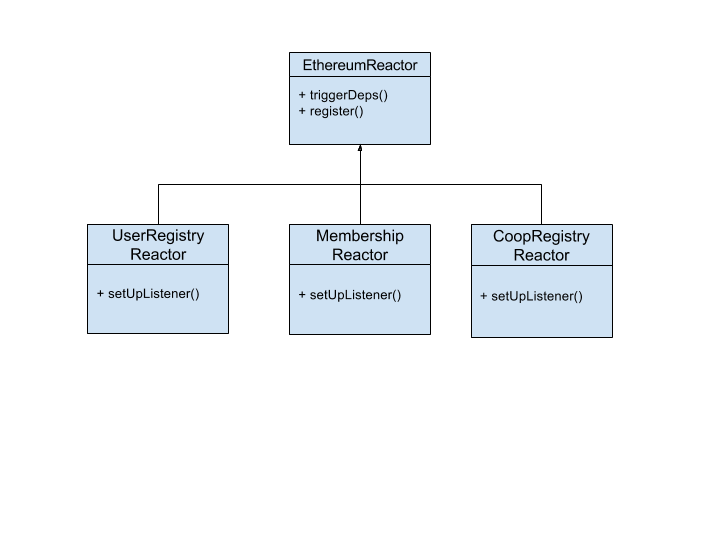
\includegraphics[width=\textwidth]{Figures/ReactorsClassDiagram}
\decoRule
\caption[]{Class diagram for Ethereum reactor classes.}
\label{fig:ReactorsClassDiagram}
\end{figure}

Figure \ref{fig:ReactorsClassDiagram} shows the class hierarchy for the various reactor classes. There are currently three reactor classes; one for each of the three registries in the smart contract system: \code{UserRegistryReactor}, \code{CoopRegistryReactor} and \code{MembershipReactor}. Each reactor extends the \code{EthereumReactor} class which defines common methods between all reactors for registering and triggering dependencies. \\

\begin{figure}
\centering
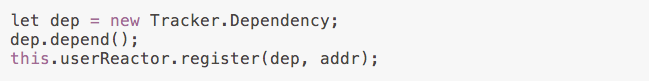
\includegraphics[width=\textwidth]{Figures/UsersDepRegistration}
\decoRule
\caption[]{Snippet of Users collection highlighting reactive dependency registration process}
\label{fig:UsersDepRegistration}
\end{figure}

Figure \ref{fig:UsersDepRegistration} is a snippet from the \code{Users} database collection. It shows how the database becomes a reactive data source through creating a reactivity dependency and registering it with the \code{CoopRegistryReactor}. \\

An alternative approach to tracking reactivity dependencies manually would be to use an in browser database such as Minimongo (this is the approach taken by other dapps such as Boardroom). Minimongo collections are built specifically as reactive database sources for use in Meteor applications. Writing the data from the backend into Minimongo collections would remove the need to manually handle reactive dependencies at such a low level. The problem with Minimongo is that collection updates would not sync automatically with the Web3 backend. Write and delete operations would have to be duplicated; once for the Minimongo collection and once for the web3 backend. Although automatic reactivity would be convenient, trying to maintain two separate data stores consistently is an easy way to introduce bugs and has so far been avoided.\\

\subsection{User Interface}
The Go-op UI (User Interface) is divided into several views (see section). Each view is defined by a HTML template and a javascript controller. When Meteor builds the application is compiles the HTML templates into javascript objects. The view controllers use the Meteor Template library to access the compiled template objects. Template objects provide a number of different methods for executing functionality at different stages of a template lifecycle including a way to attache template helpers and event handlers. The actual rendering of templates is handled by the Blaze template engine. \\

Thanks to the database layer that has just been discussed, all of the logic in the view controllers is relatively simple. Data is retrieved from the 'database' and then used to render the template. Because the database is implemented as a reactive data source and, by default, template helpers as reactive data contexts, the view controller logic doesn't really have to worry about reactivity at all. When a reactive computation context needs to be created explicitly, such as within the template onCreated function, the Tracker library is used. \\

\subsection{User Experience}
User experience is extra important for blockchain based applications because of the significant delays introduced by transaction confirmation times. Users are accustomed to fast response times so creating an application that responds quickly but doesn't make preemptive mistakes can be difficult. As Go-op is a proof of concept application user experience has not been the top priority. Nevertheless, a few optimisations have been made and possible improvements considered.\\

The first step to improving response times is to minimise the number of separate transactions needed to perform one logical process. Initially, the process of creating a new coop took three transactions. The first one deployed a new CoopContract, the second added the Coop to the CoopRegistry and the final transaction added the creator as the first member. A new block is mined roughly every seventeen seconds on the Ethereum network and given that transactions often don't make it the next block straight away, it could potentially take well over a minute for the application to confirm a new coop being created. This process was improved somewhat and now only takes two transactions to complete. This was achieved by adding the contract creation logic into the CoopRegistry and exposing a newCoop method. Theoretically, there is really no reason why the whole process cannot be performed in one transaction. It could be done fairly simply by adding more application controller contracts on top of the registry contracts. Although the return type problem (discussed in section ) means that it is currently not possible to expose a pubic API entirely through top level contracts (still need direct access to registries) redesigning the Go-op smart contract system this way would probably have a lot of benefits including minimising transactions, helping consistency and simplifying front end code.\\

Reducing the number of transactions is useful but even waiting for one transaction to process is pretty unacceptable for UX. The best way around this is an optimistic interface. An optimistic interfaces would update the UI in response to user input before confirmation is received from the blockchain. Ideally, icons would be used to indicate which parts of the application are pending and not yet confirmed. Optimistic UIs work best when there is a high degree of confidence in that the request to the backend will succeed. Given the high availability of blockchain networks it is probably possible to have quite a high degree of certainty about the behaviour of Ethereum contracts. Go-op doesn't currently implement an optimistic UI.\\

\myworries{TODO -.Loading animations}

\subsection{Deployment Script}
\label{subsec:deployScript}
The deployContracts script is used to both compile and deploy smart contracts. \\

A distinction can be made between what might be termed 'static' and 'dynamic' smart contracts within a smart contract system. Static contracts serve as entry points to the Ethereum backend. The address of these contracts needs to be known by the front end in advance. The CoopRegistry is an example of a static contract. Dynamic contracts are created on the fly during application usage. The CoopContract is an example of a contract that is created dynamically. \\

In either case, whether contracts are static or dynamic the front end needs to know the contract ABI (application binary interface) so it can create a 'handle' for interaction or deployment with the web3 library.\\

With this in mind, the purpose of the deployContracts script is two fold. It's first purpose is to compile each of the Solidity contracts and wrap the resulting ABI into modules so that they can be loaded by the front end code. Figure X shows an example output for a compiled CoopRegistry contract. The second purpose of the deployContracts script it to deploy the contracts. Only the static contracts need to be deployed by this script i.e no CoopContracts need to be deployed here. Once the static contracts have been deployed they must also be registered with the CMC (see information about CMCs see section). Finally, the addresses of the deployed contracts are written to the contractLocations module so that they can also be accessed by the front end code. \\

